%%%%%%%%%%%%%%%%%%%%%%%%%%%%%%%%%%
%    Introduction                %
%%%%%%%%%%%%%%%%%%%%%%%%%%%%%%%%%

%1. Definition of polyolefin 
%2. proportions of polyolefin in the production of plastic per year 
%3. Why polyolefin are so popular ? 
%    a. chemical composition of crude oil and natural gas 
%    b. properties of polyolefins + Stability 
%    c. the process 
%4. main applications of polyolefins

\begin{frame}{Definition of Polyolefins (PO)}
    % polyolefin are made by polycondension of alkene 
    \begin{figure}
        \centering
        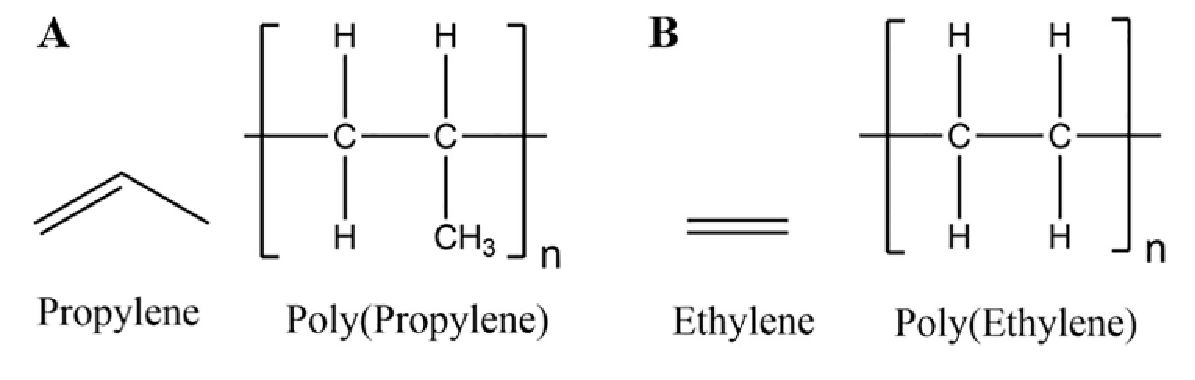
\includegraphics[width = 0.8\textwidth]{Figures/1_PO.pdf}
        \caption{Monomer and polymer of (A) PP and (B) PE \cite{jubinville_comprehensive_2020}.}
    \end{figure}
\end{frame}

\begin{frame}{PO represent 40\% of the world plastic production}
    \begin{figure}
        \centering
        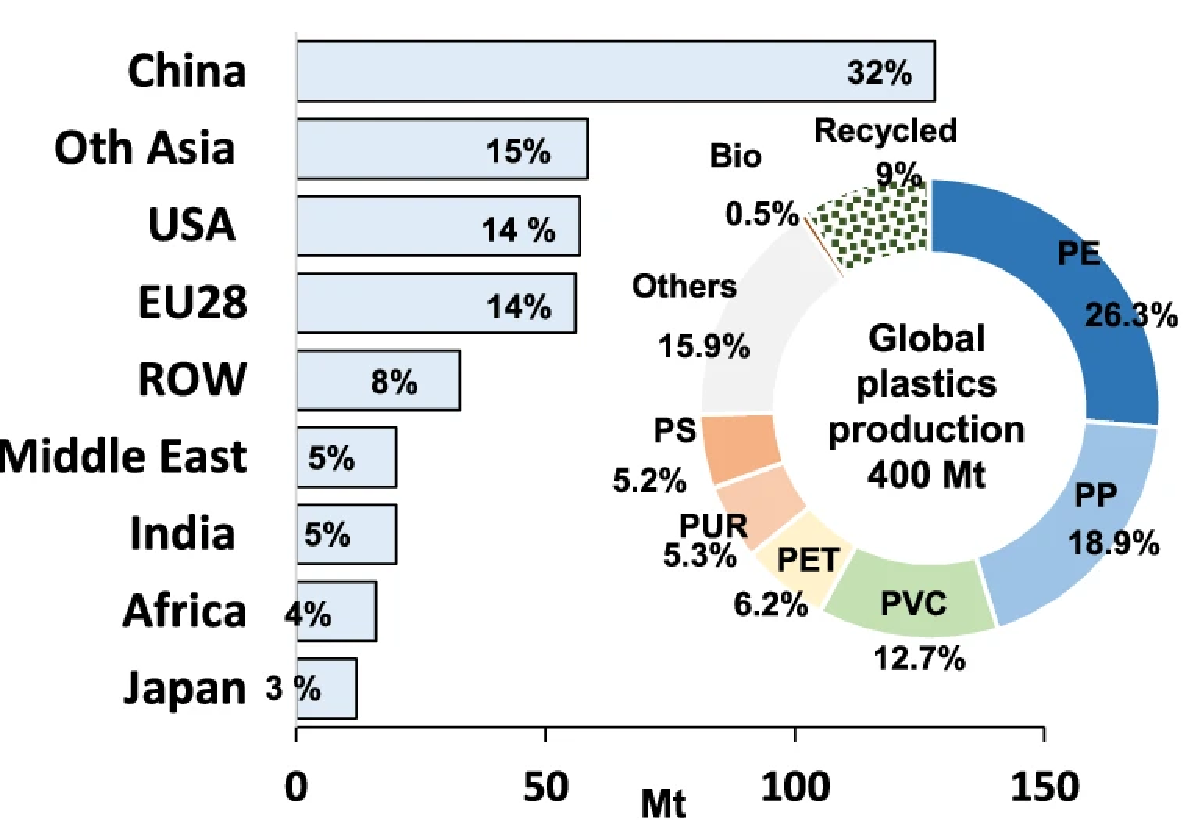
\includegraphics[width = 0.5\textwidth]{Figures/2_platci_production.pdf}
        \caption{Global plastic production breakdown by region/type \cite{houssini_complexities_2025}}
    \end{figure}
\end{frame}

\begin{frame}{Why polyolefin are so popular ?}
    % "1 barrel crude → 15% naphtha → steam cracker → 40–50% light alkenes → PE/PP
    % Naphtha is a volatile, flammable liquid mixture constituting 15-30% of crude oil by weight, typically boiling between 30°C and 200°C
    \begin{figure}
            \centering
            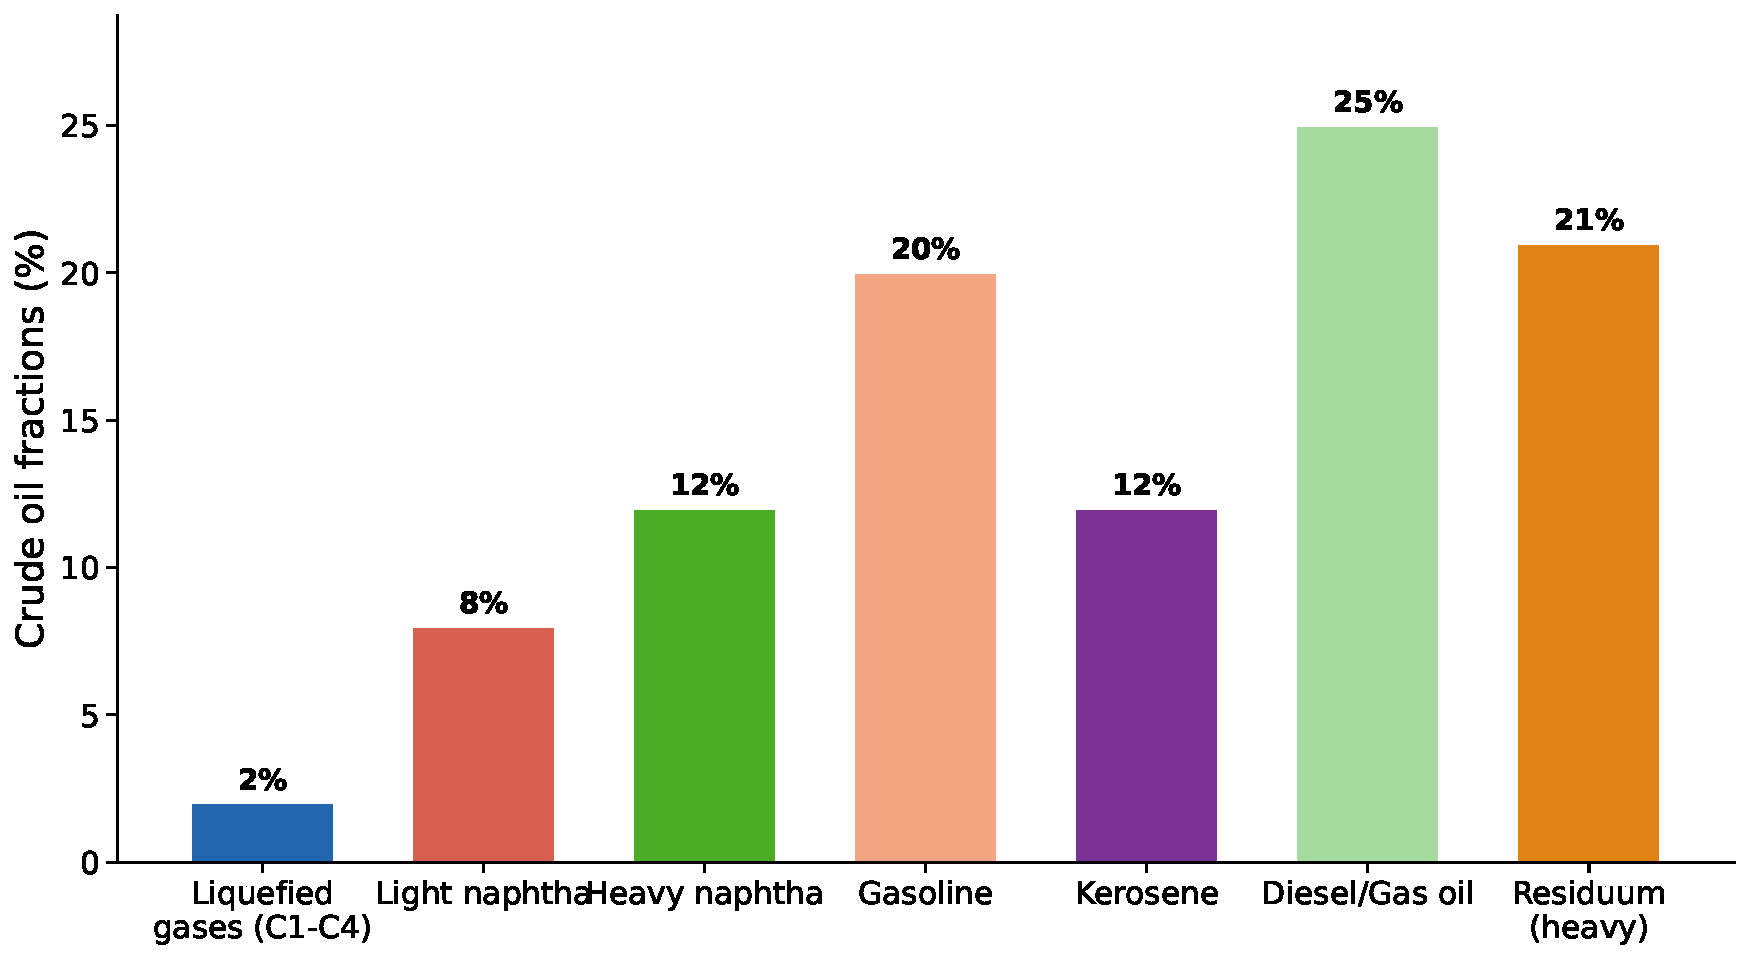
\includegraphics[width = 0.6\textwidth]{Figures/4_crude_oil.pdf}
            \caption{Atmospheric distillation of crude oil \cite{noauthor_crude_2026}}
        \end{figure}
    Naphtha $\rightarrow$ Ethylene, propylene \textbf{or} gasoline (oct. 95 or+) depending on the \textbf{Market}. 
%Competition between (i) Steam cracking and (ii) catalytic reforming
\end{frame}

\begin{frame}{because the raw materials are cheap}
    \begin{block}{}
        Naphtha + H₂O (steam) → Furnace (850°C) $\rightarrow$ Ethylene (30\%) + Propylene (16\%) + $H_2$ + $CH_4$ + C4s + BTX + coke
    \end{block}
     \begin{figure}
            \centering
            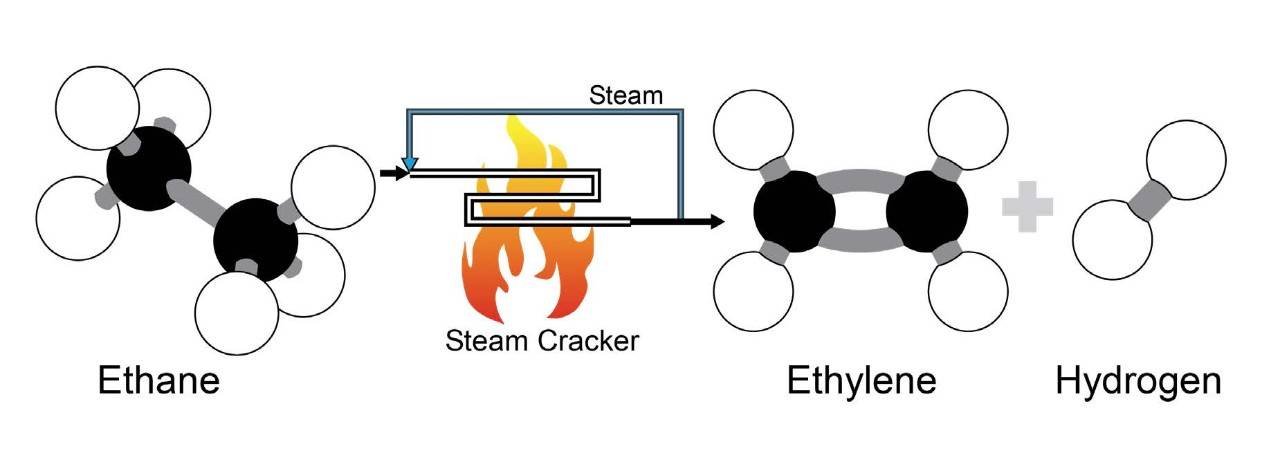
\includegraphics[width = 0.4\textwidth]{Figures/cracking.jpg}
            \caption{Formation of ethylene from ethane ($C_2H_6$) \cite{noauthor_clendenin_nodate}}
        \end{figure}
    \begin{alertblock}{natural gas (95\% $CH_4$ + 3\% $C_2H_6$)}
        can also be converted into Ethylene with higher yield (shale gas of US Gulf cost). \cite{noauthor_composition_nodate}
        % US produce 70% from natural gas while EU only 10% 
     \end{alertblock}
\end{frame}
 
%Low density: 0.91–0.96 g/cm³ (floats, light)
%Chemical resistance: Acids, bases, solvents
%Temp range: -100°C to +80°C continuous
%Processable: Injection, blow molding, extrusion, film blowing
%Recyclable: #2 plastic (though only ~10% recycled)
%Cost: $1,200–1,800/tonne (2026 avg)
%
\begin{frame}{Because PO are versatile}
    \begin{minipage}{0.45\textwidth}
        \textbf{PP (Polypropylene)}
        \begin{itemize}
            \item $M_w$
            \item Tacticity
            
        \end{itemize}
    \end{minipage}
    \hfill
    \begin{minipage}{0.45\textwidth}
        \textbf{PE (Polyethylene)}
        \begin{itemize}
            \item $M_w$
            \item PDI
            \item Branching 
        \end{itemize}
    \end{minipage}
    \begin{block}{for thermoplastics}
        $M_w + \text{ PDI } + \text{ branching } + \text{ Tacticity } = \xi_c$ \& properties ($E$,$\rho$ $\sigma$  and $T_g$) 
    \end{block}
    \begin{alertblock}{trade off}
    PE density knob $\rightarrow$ HDPE pipes vs LDPE films \\ 
    PP tacticity knob $\rightarrow$ Homo (stiff) vs Copo (tough)
    \end{alertblock}
\end{frame}

% chemical resistance 

\begin{frame}{PO exhibit excellent chemical resistance}
    \begin{figure}
        \centering
        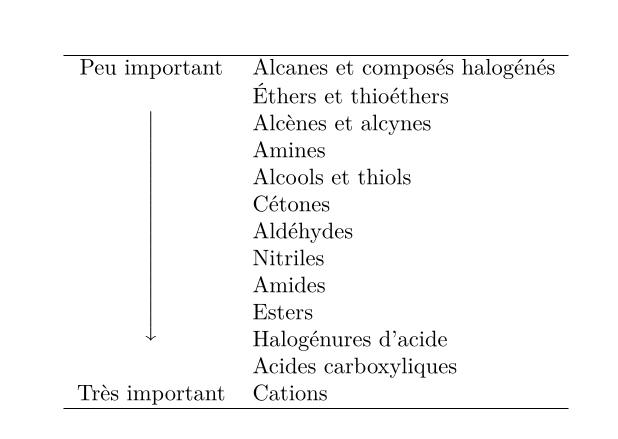
\includegraphics[width = 0.5\textwidth]{Figures/5_reactivité.png}
        \caption{Functional group reactivity (adapted from LMAPR1230).}
    \end{figure}
\end{frame}

\begin{frame}{Summary of PP/PE properties}
    \begin{minipage}{0.48\textwidth}
        \textbf{PE (Polyethylene) \cite{hughes_polyethylene_2023}}
        \vspace{0.2cm}
        \begin{block}{Key Advantages}
            \begin{itemize}
                \item Low density: 0.91--0.97 g/cm$^3$
                \item Chemical resistance: Excellent (acids, bases, solvents)
                \item Temp range: -100°C to +130°C (HDPE), +80°C continuous
                \item Processable: Injection, blow molding, extrusion, film blowing
                \item Cost: \$1,200--1,800/tonne (2026 avg)
                \item \textbf{Tunable}: Density (stiffness), MFI 0.1--50
            \end{itemize}
        \end{block}
    \end{minipage}%
    \hfill
    \begin{minipage}{0.48\textwidth}
        \textbf{PP (Polypropylene) \cite{hughes_polyethylene_2023}}

        \vspace{0.2cm}
        \begin{block}{Key Advantages}
            \begin{itemize}
                \item Low density: 0.90--0.91 g/cm$^3$ 
                \item Chemical resistance: Excellent (acids, bases, oils)
                \item Temp range: 0°C to +140°C 
                \item Processable: Injection molding, extrusion, fibers
                \item Cost: \$1,100--1,600/tonne (2026 avg)
                \item \textbf{Tunable}: MFI 0.3--100, copolymer \% (impact)
            \end{itemize}
        \end{block}
    \end{minipage}
\end{frame}


    
     


\begin{frame}{PO is mainly used for short-term usage}
    \begin{figure}
            \centering
            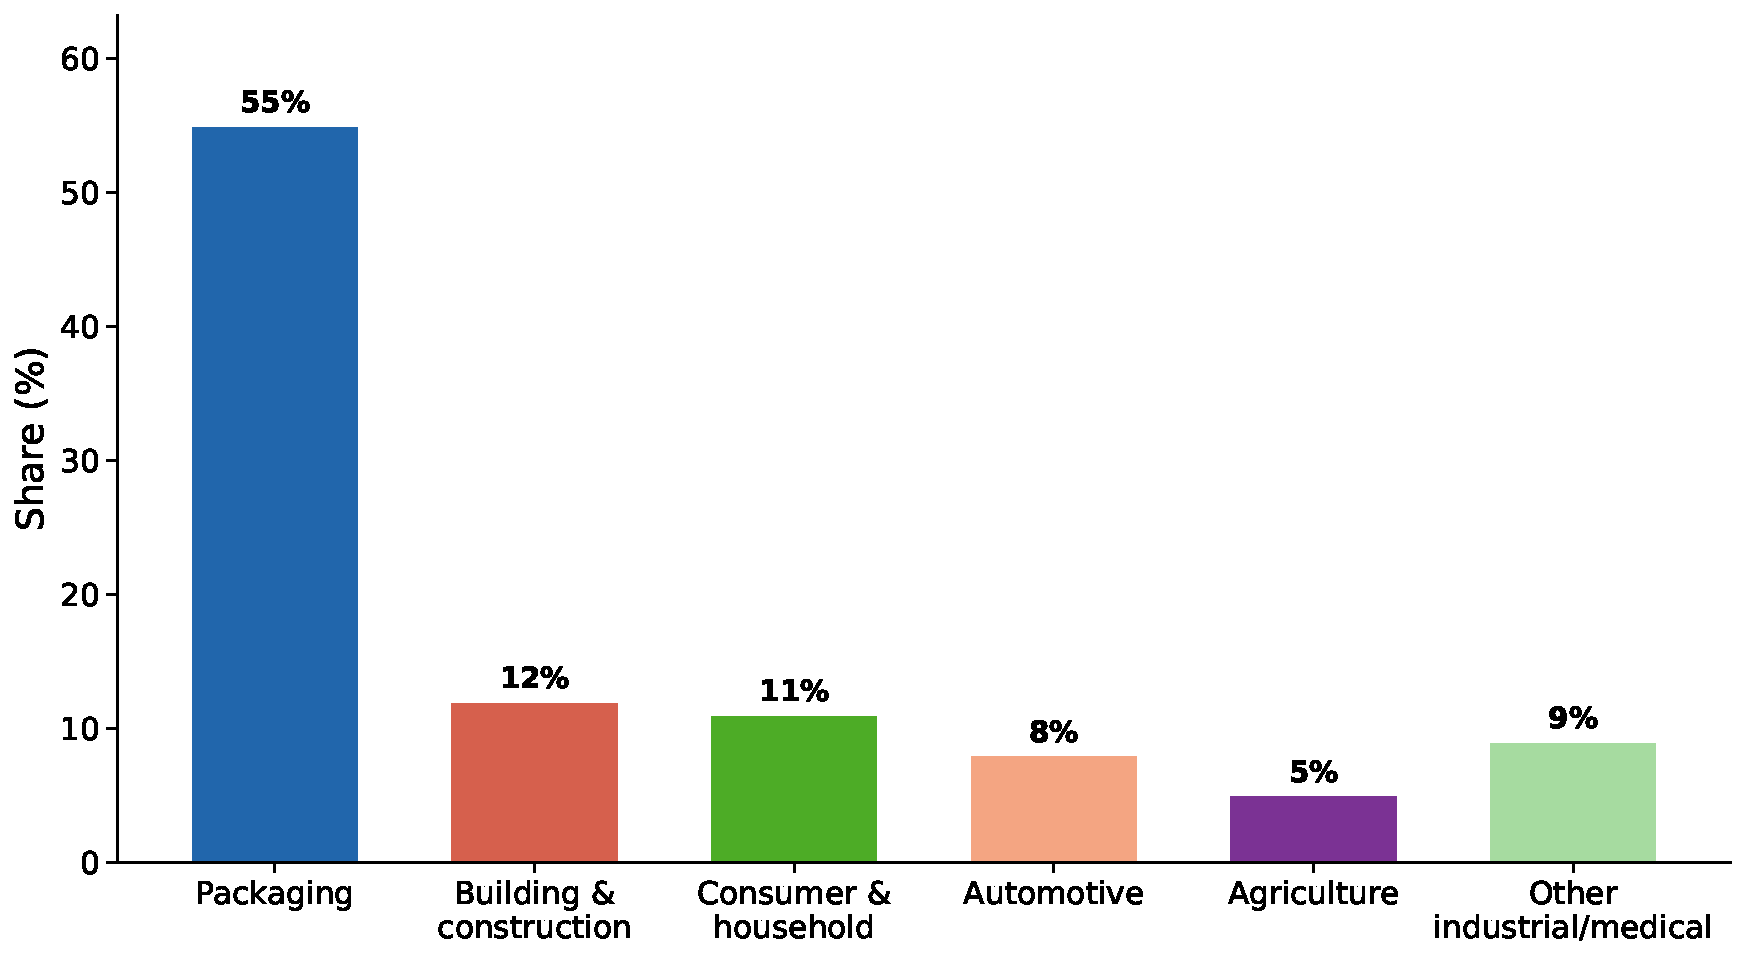
\includegraphics[width = 0.7\textwidth]{Figures/3_PO_use.pdf}
            \caption{PO per final use \cite{pcep2018}}
        \end{figure}
\end{frame}
